\documentclass{article}

\usepackage[utf8]{inputenc}

\usepackage{amsmath}
\usepackage{graphicx}
\usepackage{amssymb}
\usepackage{float}

\setlength{\parskip}{\baselineskip}%
\setlength{\parindent}{0pt}%

\begin{document}

\title{Boundary Layers}
\author{lwp26 }
\date{October 2022}
\maketitle

\section{Abstract}
In this report data collected from air in a wind tunnel will be analysed to determine the
velocity profile of the air and investigate the effects of the boundary layer on laminar and turbulent flow.
The boundary layers of spheres of varying mass and size were also investigated by calculating drag force and downards velocity
of a sphere is falling in vertical fluid collumns of different viscosities.

\section{Introduction}

% Aims, Objectives and context

\subsection{Aims}

\begin{itemize}
\item To gather flow data and calculate velocity profiles for both laminar and turbulent flows.
\item To analyse and compare the flow velocity profiles of laminar and turbulent flows to gain an understanding of boundary layers
\item To compare drag coefficients and Reynolds numbers of spheres of varying mass and size through fluids of varying viscosity to gain further understanding of boundary layers.
\end{itemize}

\section{Methodology}

% Summary of theory and information to reproduce
\subsection{Flow velocity profiles}
The velocity profiles were determined using a wind tunnel with 2 manometers. One manometer's pitot probe was placed far away from the wall and was used to measure $V_\infty$ The other manometer's pitot probe's position was varied to record $V$ at $x$ mm from the wall.

From Bernouli's equation
\begin{equation}
    p_0 - p = \frac{1}{2}\rho_a u^2 = \rho_l g \Delta h sin \theta
\end{equation}
After rearanging for flow velocity, $u$, equation (1) becomes
\begin{equation}
    u = \sqrt{ \frac{2 \rho_l g \Delta h sin \theta}{\rho_a} }
\end{equation}
Which means the ratio of flow velocities becomes
\begin{equation}
    r_u = \frac{u}{U_\infty} = \sqrt{\frac{\Delta h}{\Delta h_\infty}}
\end{equation}
The Reynolds number of a flow is a dimensionless quantity used to distuinguish between laminar and turbulent flow.
It can be calculated using the equation below
\begin{equation}
    R_e = \frac{\rho_l u L}{\mu}
\end{equation}
At high Reynolds numbers, typically $R_e > 10^5$ for a flat plate, the flow transitions from laminar to turbulent.

The momentum flux is the rate of momentum transfer per unit area. It is given by
\begin{equation}
    \dot{M} = \int_0^\infty (U_{\infty} - u) \rho u dy = \int_0^\infty \rho U_{\infty}^2 \left( 1 - \frac{u}{U_{\infty}} \right) \left( \frac{u}{U_{\infty}} \right) dy
\end{equation}

\subsection{Drag coefficient of spheres}

The drag coefficient of an aerofoil is a dimensionless quantity used to quantify how aerodynamic an object is.
\begin{equation}
    C_D = \frac{F_D}{\frac{1}{2}\rho_l U^2 L}
\end{equation}
For the case of falling vertically in a fluid the drag force $F_D$ can be calculated using the weight and upthrust as seen below
\begin{equation}
    C_D = \frac{mg - \rho V g}{\frac{1}{2}\rho_l U^2 L}
\end{equation}

\section{Results}

\subsection{Flow profiles}

\begin{figure}[H]
\centering
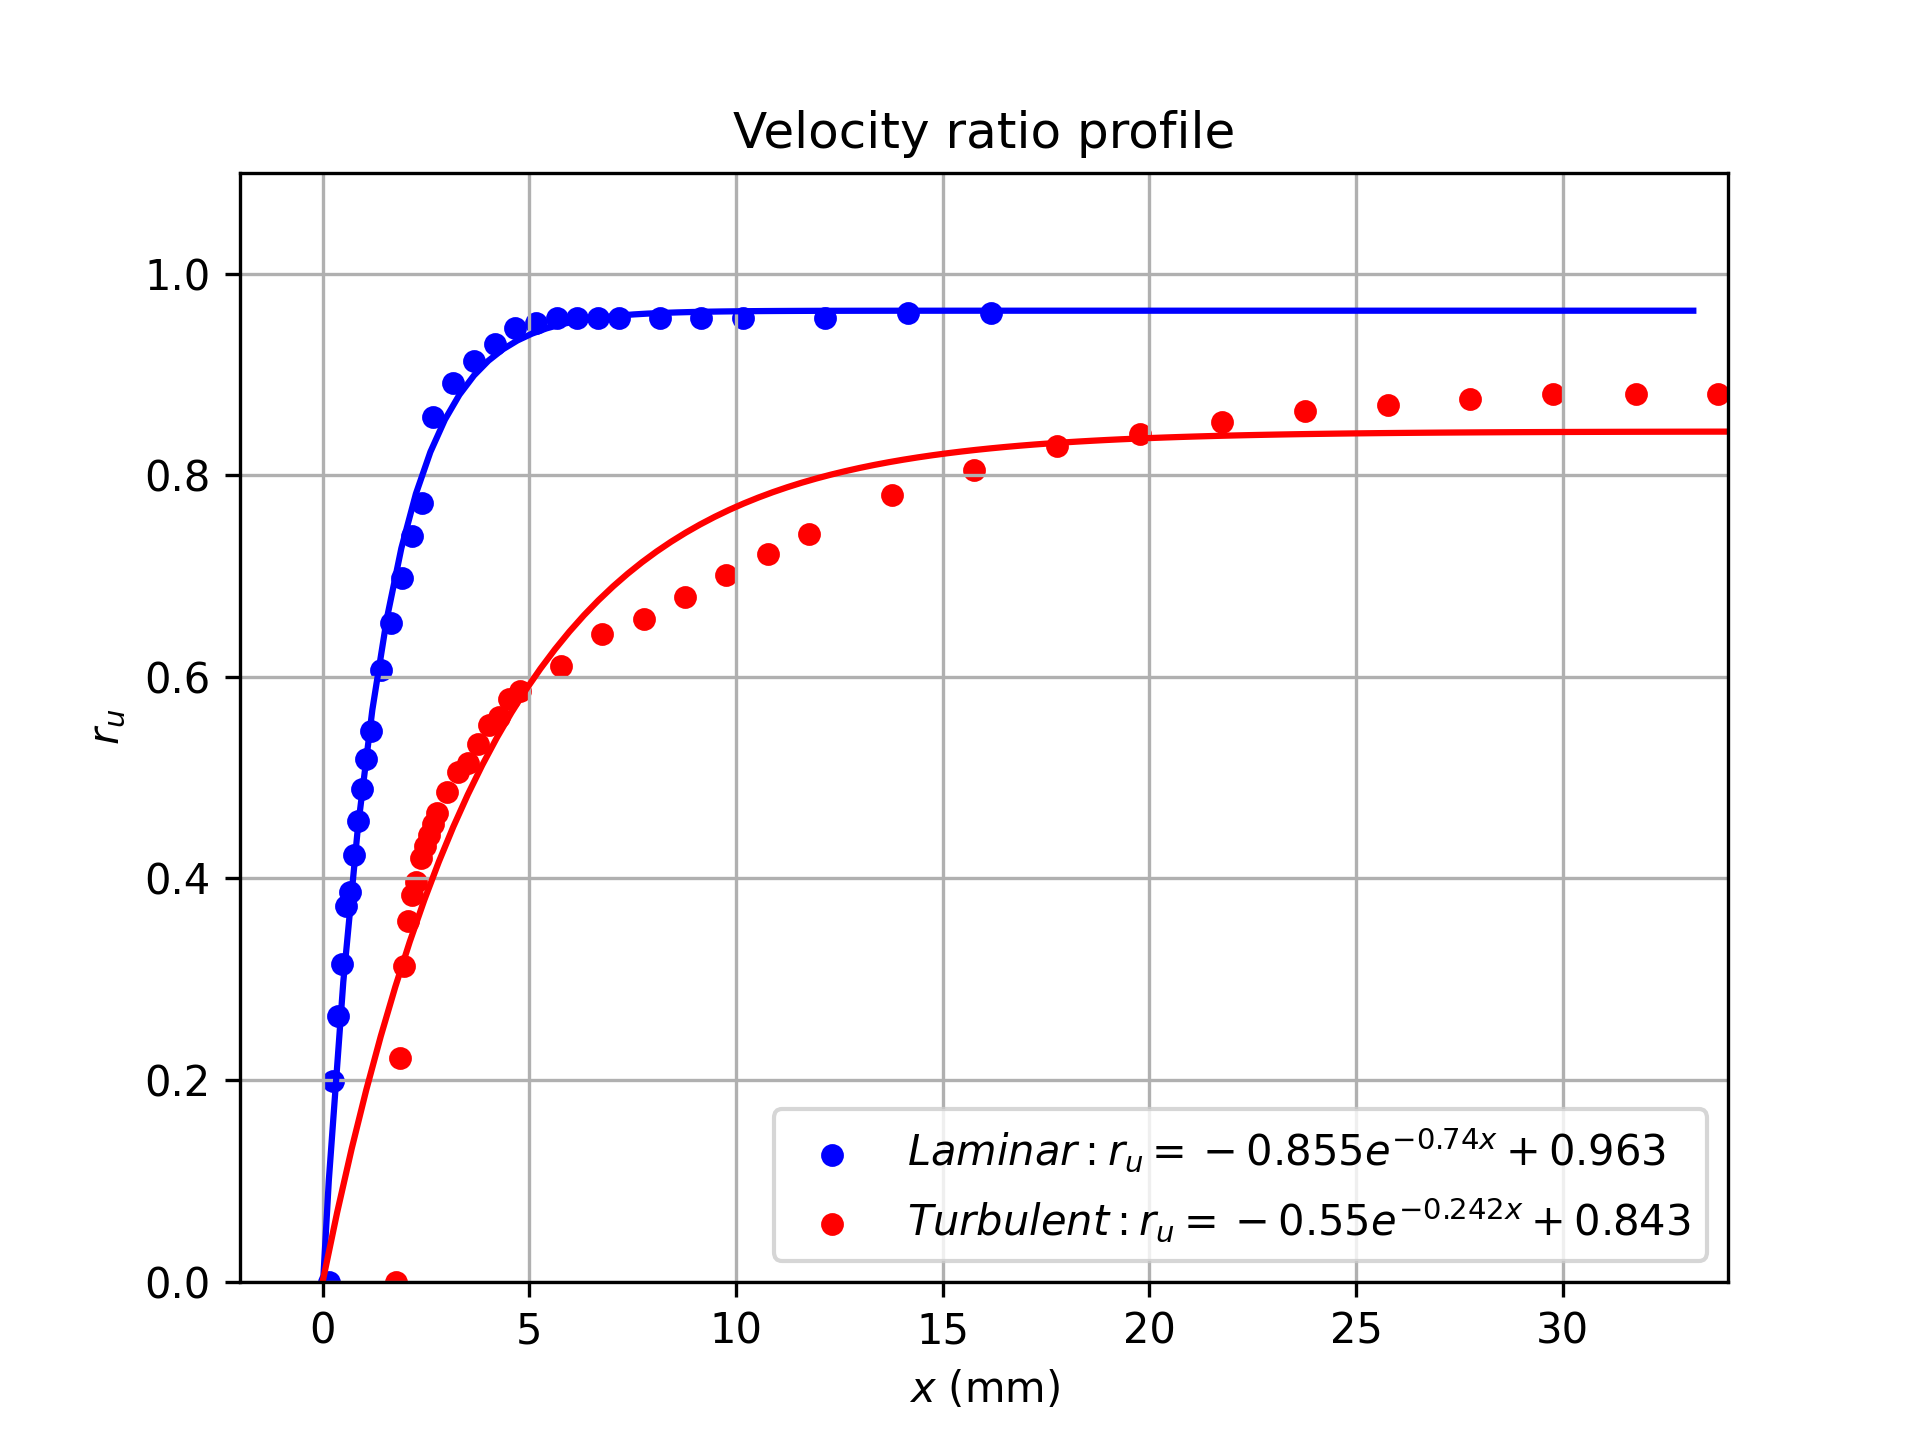
\includegraphics[width=1\textwidth]{velocity_profiles.png}
\caption{\label{fig:velocity_profiles} Graph of the laminar and turbulent flow profiles}
\end{figure}

\begin{figure}[H]
\centering
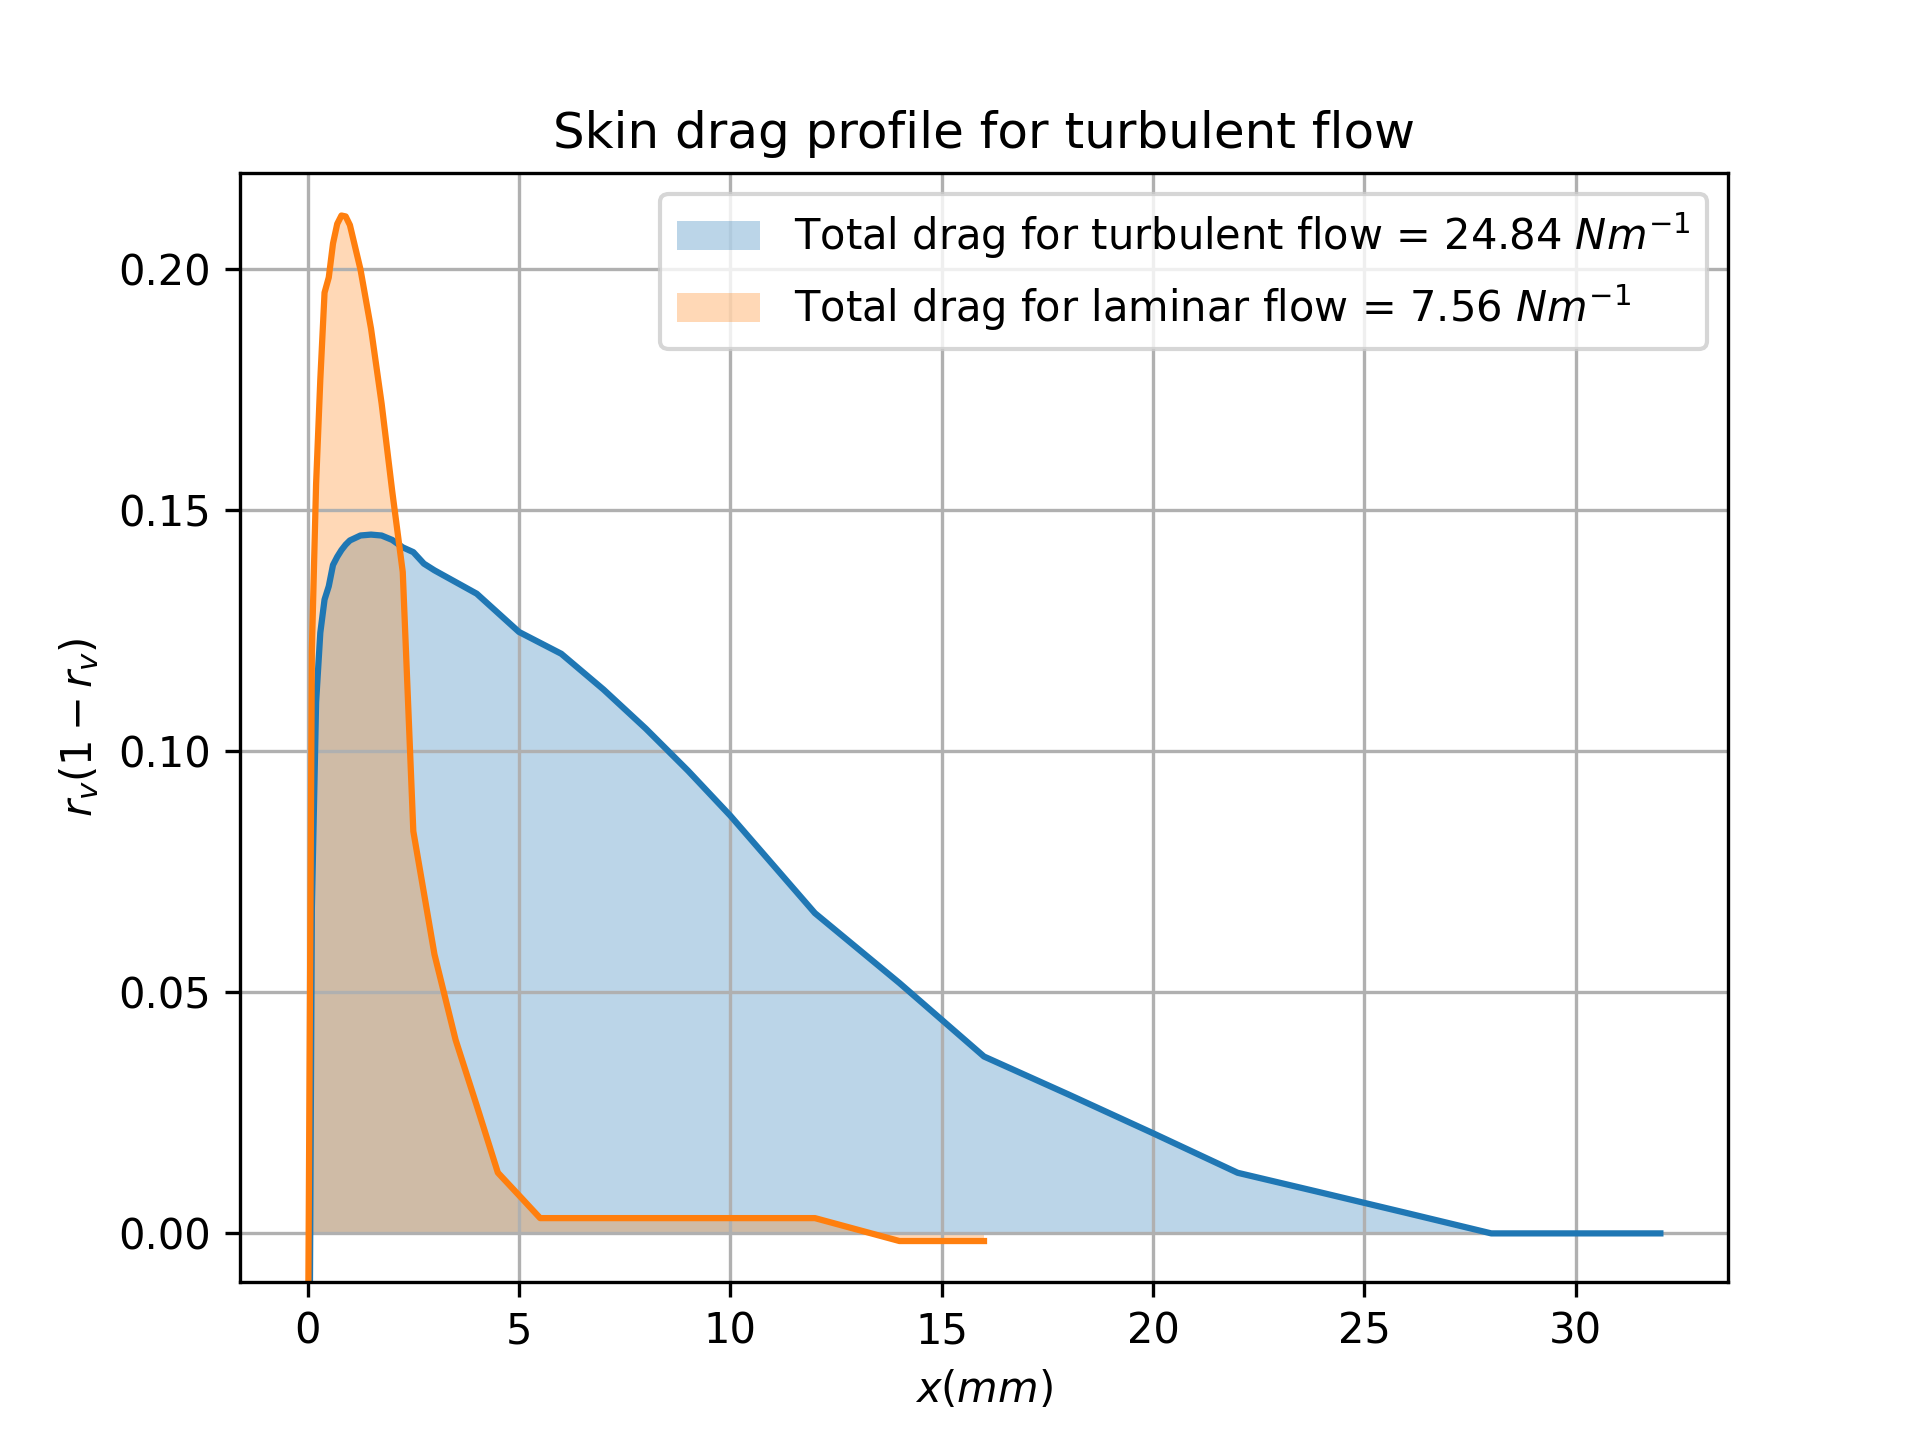
\includegraphics[width=1\textwidth]{drag_profiles.png}
\caption{\label{fig:drag_profiles} Graph of the turbulent skin drag profile and total drag force per unit height of wall from equation (5)}
\end{figure}

\subsection{Drag Coefficients}

\begin{center}
\begin{tabular}{|c|c|c|c|c|c|c|c|c|}
\hline
Fluid & Mass & Diameter & Time & $U$ & $F_u$ & $F_D$ & $C_D$ & $Re$ \\
- & g & mm & s & m/s & N & N & - & - \\
\hline
Water & $2.426$ & $15.63$ & $5.0$ & $0.205$ & $0.0196$ & $0.0042$ & $0.86$ & $3204$ \\
Glycerol & $8.439$ & $12.65$ & $0.8$ & $1.28$ & $0.0131$ & $0.0697$ & $0.085$ & $13.51$ \\
Oil & $1.453$ & $12.60$ & $8.2$ & $0.125$ & $0.0089$ & $0.0053$ & $3.93$ & $28.14$ \\
Water & $2.325$ & $15.41$ & $5.1$ & $0.201$ & $0.0188$ & $0.0040$ & $0.88$ & $3097$ \\
\hline
\end{tabular}
\end{center}

\begin{figure}[H]
\centering
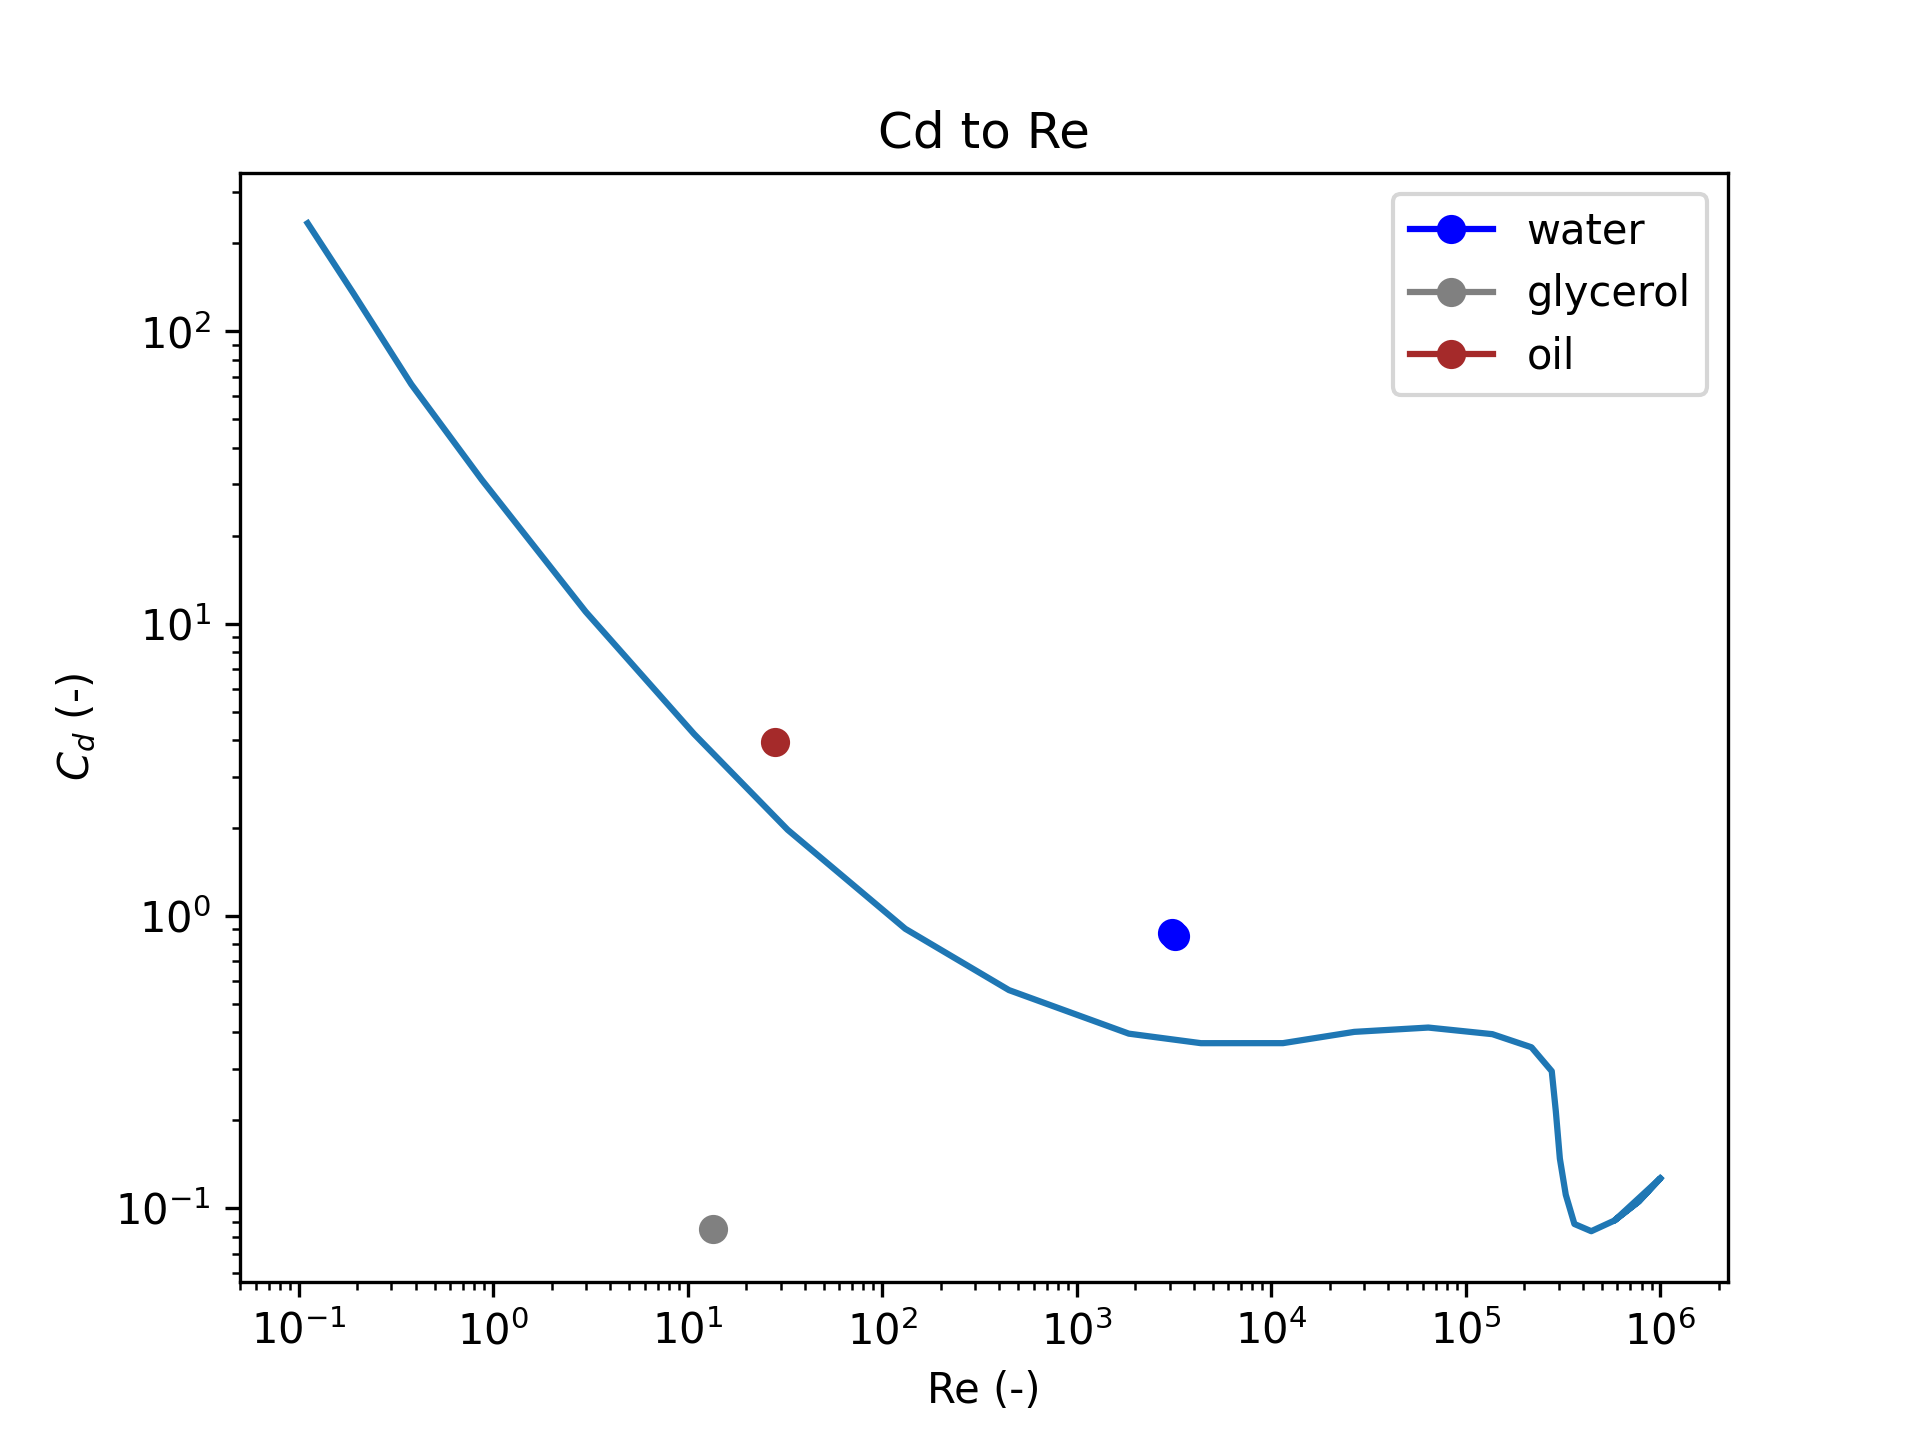
\includegraphics[width=1\textwidth]{CdRe_graph.png}
\caption{\label{fig:CdRe_graph} The drag coefficient of spheres as a function of Re}
\end{figure}

\begin{figure}[H]
\centering
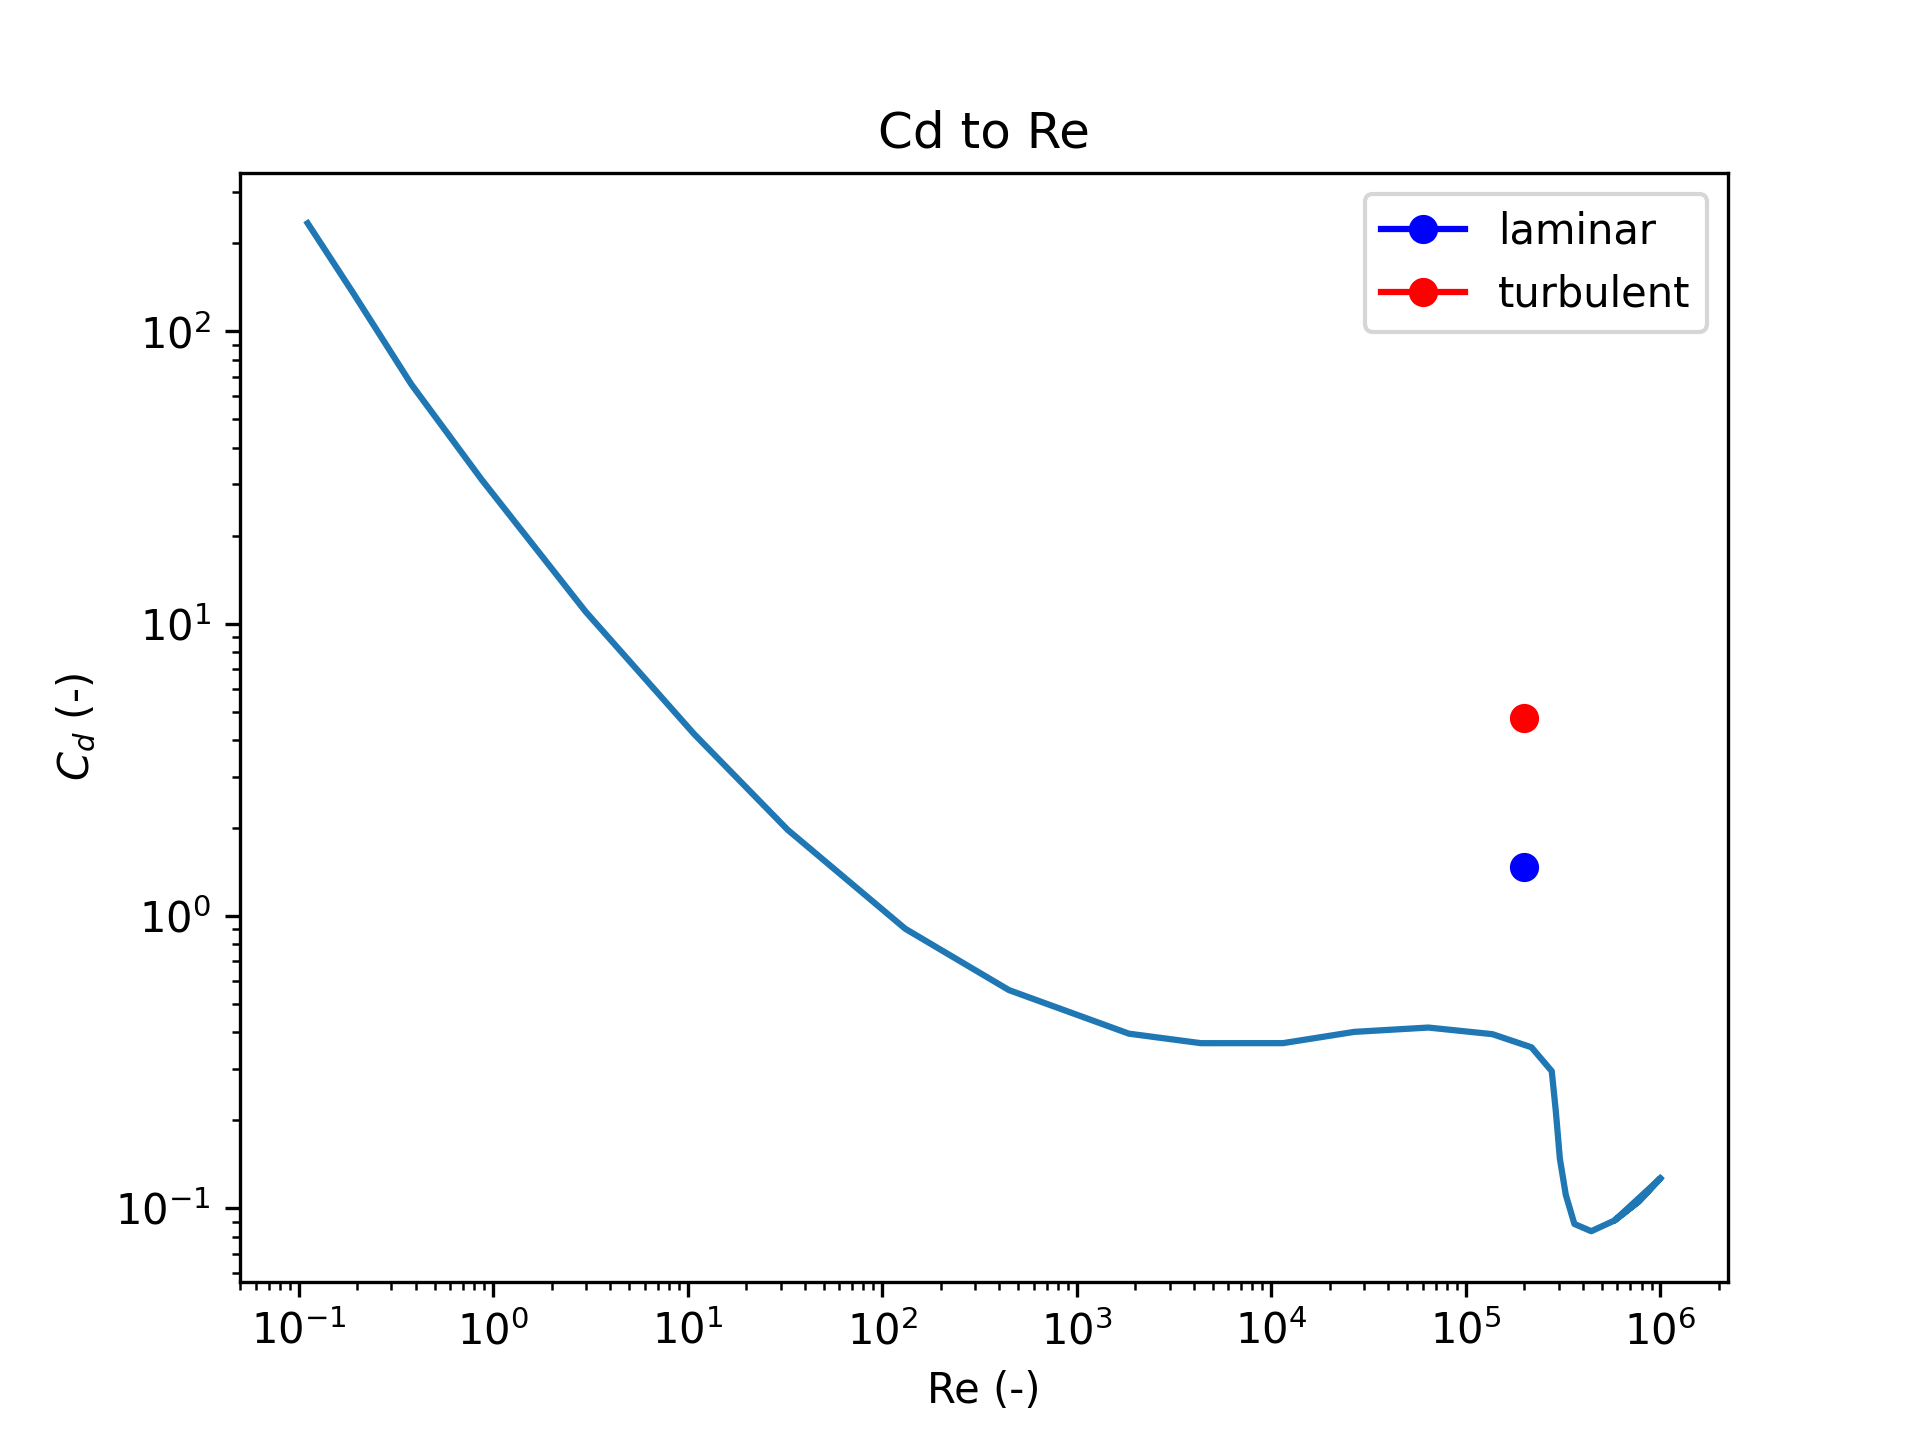
\includegraphics[width=1\textwidth]{CdRe_mloss.png}
\caption{\label{fig:CdRe_mloss} The drag coefficient of spheres as a function of Re}
\end{figure}

\section{Discussion}

The laminar free stream velocity was calculated to be $3.38$ m/s and the 
turbulent free stream velocity was calculated to be $3.4$ m/s, The Reynolds number
for these flows were $1.70\times 10^6$ and $1.71 \times 10^6$ respectively.

Figure \ref{fig:velocity_profiles} shows that the turbulent boundary layer
is much thicker than the laminar boundary layer the velocity increases over a
longer distance to reach the free stream velocity. 
It was observed using the microphone that the turbulent flow was louder than laminar flow.
This is because turbulent flow has more pressure and velocity fluctuations than laminar flow.

The graphs in figure \ref{fig:drag_profiles} shows that the skin drag profiles for laminar and turbulent flow.
Using equation (5) the total drag force per unit height of wall was calculated to be $ 7.56 $ $Nm^{-1}$ and
$ 24.84 $ $Nm^{-1}$ for laminar and turbulent flow respectively.
It can also be seen that the laminar drag profile has a sharp peak all within 5mm of the wall, 
whereas the turbulent drag profile has a lower peak but far more drag further away from the wall.
This again shows that the turbulent boundary layer is much thicker than the laminar boundary layer.

Another method to calculate the skin friction at the surface of the wall was to use the
gradient of the velocity profile at the wall multiplied by the viscocity of the fluid.
\begin{equation}
    \tau = \mu \frac{du}{dx}
\end{equation}
The skin friction was calculated to be $ 0.12 $ $Nm^{-2}$ and $ 0.14 $ $Nm^{-2}$ for laminar and turbulent flow respectively.
These values are much lower than the values calculated using equation (5)

Figure \ref{fig:CdRe_graph} shows the 4 spheres on the graph of standard drag coefficients 
against Reynolds numbers. It follows an initial linear trend before becoming more curved due to turbulent effects.
The sudden drop in drag coefficient is due to the boundary layer in front of the sphere
becomming thinner and the flow transitions into turbulent.

Figure \ref{fig:CdRe_mloss} shows the drag coefficient of the turbulent and laminar
boundary layers using the rate of momentum loss to calculate drag coefficients on the graph 
of standard drag coefficients against Reynolds numbers.

%interpret results and comment on anomalies

\section{Conclusion}

From the experimental data gathered, the laminar and turbulent velocity profiles were calculated
and graphically displayed to show the differences in profiles of the two flows. As expected the laminar flow had a much thinner 
boundary layer than the turbulent flow. It was also shown through theory and later analysis, 
that the turbulent flow had higher skin drag force than the laminar flow. It was also shown
that spheres at higher reynolds numbers had lower drag coefficients than spheres at lower reynolds numbers.


\end{document}